% Options for packages loaded elsewhere
\PassOptionsToPackage{unicode}{hyperref}
\PassOptionsToPackage{hyphens}{url}
%
\documentclass[
  ignorenonframetext,
  aspectratio=169,
]{beamer}
\usepackage{pgfpages}
\setbeamertemplate{caption}[numbered]
\setbeamertemplate{caption label separator}{: }
\setbeamercolor{caption name}{fg=normal text.fg}
\beamertemplatenavigationsymbolsempty
% Prevent slide breaks in the middle of a paragraph
\widowpenalties 1 10000
\raggedbottom
\setbeamertemplate{part page}{
  \centering
  \begin{beamercolorbox}[sep=16pt,center]{part title}
    \usebeamerfont{part title}\insertpart\par
  \end{beamercolorbox}
}
\setbeamertemplate{section page}{
  \centering
  \begin{beamercolorbox}[sep=12pt,center]{part title}
    \usebeamerfont{section title}\insertsection\par
  \end{beamercolorbox}
}
\setbeamertemplate{subsection page}{
  \centering
  \begin{beamercolorbox}[sep=8pt,center]{part title}
    \usebeamerfont{subsection title}\insertsubsection\par
  \end{beamercolorbox}
}
\AtBeginPart{
  \frame{\partpage}
}
\AtBeginSection{
  \ifbibliography
  \else
    \frame{\sectionpage}
  \fi
}
\AtBeginSubsection{
  \frame{\subsectionpage}
}

\usepackage{amsmath,amssymb}
\usepackage{lmodern}
\usepackage{iftex}
\ifPDFTeX
  \usepackage[T1]{fontenc}
  \usepackage[utf8]{inputenc}
  \usepackage{textcomp} % provide euro and other symbols
\else % if luatex or xetex
  \usepackage{unicode-math}
  \defaultfontfeatures{Scale=MatchLowercase}
  \defaultfontfeatures[\rmfamily]{Ligatures=TeX,Scale=1}
\fi
\usetheme[]{Madrid}
\usecolortheme{DarkBlue}
% Use upquote if available, for straight quotes in verbatim environments
\IfFileExists{upquote.sty}{\usepackage{upquote}}{}
\IfFileExists{microtype.sty}{% use microtype if available
  \usepackage[]{microtype}
  \UseMicrotypeSet[protrusion]{basicmath} % disable protrusion for tt fonts
}{}
\makeatletter
\@ifundefined{KOMAClassName}{% if non-KOMA class
  \IfFileExists{parskip.sty}{%
    \usepackage{parskip}
  }{% else
    \setlength{\parindent}{0pt}
    \setlength{\parskip}{6pt plus 2pt minus 1pt}}
}{% if KOMA class
  \KOMAoptions{parskip=half}}
\makeatother
\usepackage{xcolor}
\newif\ifbibliography
\setlength{\emergencystretch}{3em} % prevent overfull lines
\setcounter{secnumdepth}{-\maxdimen} % remove section numbering


\providecommand{\tightlist}{%
  \setlength{\itemsep}{0pt}\setlength{\parskip}{0pt}}\usepackage{longtable,booktabs,array}
\usepackage{calc} % for calculating minipage widths
\usepackage{caption}
% Make caption package work with longtable
\makeatletter
\def\fnum@table{\tablename~\thetable}
\makeatother
\usepackage{graphicx}
\makeatletter
\def\maxwidth{\ifdim\Gin@nat@width>\linewidth\linewidth\else\Gin@nat@width\fi}
\def\maxheight{\ifdim\Gin@nat@height>\textheight\textheight\else\Gin@nat@height\fi}
\makeatother
% Scale images if necessary, so that they will not overflow the page
% margins by default, and it is still possible to overwrite the defaults
% using explicit options in \includegraphics[width, height, ...]{}
\setkeys{Gin}{width=\maxwidth,height=\maxheight,keepaspectratio}
% Set default figure placement to htbp
\makeatletter
\def\fps@figure{htbp}
\makeatother

\definecolor{DarkBlue}{rgb}{0.05, 0.15, 0.3}
\setbeamercolor{structure}{fg=DarkBlue}
\makeatletter
\makeatother
\makeatletter
\makeatother
\makeatletter
\@ifpackageloaded{caption}{}{\usepackage{caption}}
\AtBeginDocument{%
\ifdefined\contentsname
  \renewcommand*\contentsname{Table of contents}
\else
  \newcommand\contentsname{Table of contents}
\fi
\ifdefined\listfigurename
  \renewcommand*\listfigurename{List of Figures}
\else
  \newcommand\listfigurename{List of Figures}
\fi
\ifdefined\listtablename
  \renewcommand*\listtablename{List of Tables}
\else
  \newcommand\listtablename{List of Tables}
\fi
\ifdefined\figurename
  \renewcommand*\figurename{Figure}
\else
  \newcommand\figurename{Figure}
\fi
\ifdefined\tablename
  \renewcommand*\tablename{Table}
\else
  \newcommand\tablename{Table}
\fi
}
\@ifpackageloaded{float}{}{\usepackage{float}}
\floatstyle{ruled}
\@ifundefined{c@chapter}{\newfloat{codelisting}{h}{lop}}{\newfloat{codelisting}{h}{lop}[chapter]}
\floatname{codelisting}{Listing}
\newcommand*\listoflistings{\listof{codelisting}{List of Listings}}
\makeatother
\makeatletter
\@ifpackageloaded{caption}{}{\usepackage{caption}}
\@ifpackageloaded{subcaption}{}{\usepackage{subcaption}}
\makeatother
\makeatletter
\@ifpackageloaded{tcolorbox}{}{\usepackage[many]{tcolorbox}}
\makeatother
\makeatletter
\@ifundefined{shadecolor}{\definecolor{shadecolor}{rgb}{.97, .97, .97}}
\makeatother
\makeatletter
\makeatother
\ifLuaTeX
  \usepackage{selnolig}  % disable illegal ligatures
\fi
\IfFileExists{bookmark.sty}{\usepackage{bookmark}}{\usepackage{hyperref}}
\IfFileExists{xurl.sty}{\usepackage{xurl}}{} % add URL line breaks if available
\urlstyle{same} % disable monospaced font for URLs
\hypersetup{
  pdftitle={6.2: Linear Regression},
  pdfauthor={Navona Calarco},
  hidelinks,
  pdfcreator={LaTeX via pandoc}}

\title{6.2: Linear Regression}
\author{Navona Calarco}
\date{}
\institute{The University of Toronto}

\begin{document}
\frame{\titlepage}
\ifdefined\Shaded\renewenvironment{Shaded}{\begin{tcolorbox}[borderline west={3pt}{0pt}{shadecolor}, boxrule=0pt, interior hidden, breakable, frame hidden, sharp corners, enhanced]}{\end{tcolorbox}}\fi

\begin{frame}[fragile]{Motivation}
\protect\hypertarget{motivation}{}
Throughout this Module we will be making use of the \texttt{Boston}
dataset in the R package \texttt{ISLR2}. We can install the package in R
and add it to our library:

\begin{verbatim}
install.packages("ISLR2")
library(ISLR2)
\end{verbatim}

The \texttt{Boston} dataset contains housing values in 506 Boston
suburbs along with 12 other variables associated with the suburbs. To
name a few,

\begin{itemize}
\tightlist
\item
  \texttt{rm}: average number of rooms per dwelling
\item
  \texttt{nox}: nitrogen oxides concentration (parts per 10 million)
\item
  \texttt{lstat}: percent of households with low socioeconomics status
\end{itemize}

We can take \texttt{medv}, the median value of owner-occupied homes in
\$1000s, to be the response variable \(Y\) and the 12 other variables to
be the predictors \(X = (X_1, \dots, X_{12})\).
\end{frame}

\begin{frame}{Motivation}
\protect\hypertarget{motivation-1}{}
There may be some specific question we'd like to address

\begin{itemize}
\tightlist
\item
  Is there a relationship between the 12 variables and housing price?

  \begin{itemize}
  \tightlist
  \item
    Does the data provide evidence of an association?
  \end{itemize}
\item
  Are all of the 12 variables associated with housing price?

  \begin{itemize}
  \tightlist
  \item
    Perhaps only a few of the variables have an effect on housing price.
  \end{itemize}
\item
  How accurate are the predictions for housing prices based on these
  variables?
\item
  Is the relationship between the variables and housing price linear?

  \begin{itemize}
  \tightlist
  \item
    Perhaps we can transform some variables to make the relationship
    linear.
  \end{itemize}
\end{itemize}

\alert{All of these questions can be answered using linear regression!}
\end{frame}

\begin{frame}{Simple Linear Regression}
\protect\hypertarget{simple-linear-regression}{}
\textbf{Simple linear regression} uses a \emph{single} predictor
variable \(X\) to predict a \emph{quantitative} response \(Y\) by
assuming the relationship between them is linear.
\[Y \approx \beta_0 + \beta_1 X\]

\begin{itemize}
\tightlist
\item
  \(\beta_0\) and \(\beta_1\) are the model \textbf{parameters} which
  are unknown.
\item
  \(\beta_0\) is the intercept term and \(\beta_1\) is the slope term.
\end{itemize}

We can use the training data to produce estimates \(\hat \beta_0\) and
\(\hat \beta_1\) and predict future responses

\[\hat{y} \approx \hat{\beta_0} + \hat{\beta_1} X\]
\end{frame}

\begin{frame}{Estimating the Coefficients}
\protect\hypertarget{estimating-the-coefficients}{}
Suppose we have \(n\) observations in our training data which each
consists of a measurement for \(X\) and \(Y\) represented by \[
(x_1, y_1),\ (x_2, y_2), \dots,\ (x_n, y_n)
\]

We want to find estimates for \(\hat \beta_0\) and \(\hat \beta_1\) such
that for all \(i = 1, \dots, n\) \[
y_i \approx \hat y_i
\]

where \(\hat y_i = \hat \beta_0 + \hat \beta_1 x_i\) is the prediction
for \(y_i\) given \(x_i\).

The most common method used to measure the difference between \(y_i\)
and \(\hat y_i\) is the least squares criterion. The idea being that
\alert{we want to find the $\hat \beta_0$ and $\hat \beta_1$ that give us the smallest difference}.
\end{frame}

\begin{frame}{Least Squares Criterion}
\protect\hypertarget{least-squares-criterion}{}
We define the \(i\)th \textbf{residual} to be the difference between the
\(i\)th observed response value and the \(i\)th predicted response
value: \[
e_i = y_i - \hat y_i
\]

The \textbf{residual sum of squares} (RSS) is the following \[
\operatorname{RSS} = e_1^2 + \cdots + e_n^2 
= \left(y_{1}-\hat{\beta}_{0}-\hat{\beta}_{1} x_{1}\right)^{2}+\cdots+\left(y_{n}-\hat{\beta}_{0}-\hat{\beta}_{1} x_{n}\right)^{2}
\]

\begin{block}{The RSS is minimized by the estimates below (where
\(\bar{x},\ \bar{y}\) are the sample means):}
\protect\hypertarget{the-rss-is-minimized-by-the-estimates-below-where-barx-bary-are-the-sample-means}{}
\[
\begin{aligned}
\hat{\beta}_{1}&=\frac{\sum_{i=1}^{n}\left(x_{i}-\bar{x}\right)\left(y_{i}-\bar{y}\right)}{\sum_{i=1}^{n}\left(x_{i}-\bar{x}\right)^{2}} \\
\hat{\beta}_{0}&=\bar{y}-\hat{\beta}_{1} \bar{x}
\end{aligned}
\]
\alert{So $\hat \beta_1$ and $\hat \beta_0$ definte the least squares coefficient estimates}
\end{block}
\end{frame}

\begin{frame}{Assessing the Accuracy of the Coefficient Estimates}
\protect\hypertarget{assessing-the-accuracy-of-the-coefficient-estimates}{}
Recall from section 6.1 that we assume the true relationship between the
predictor \(X\) and the response \(Y\) is \[
Y = f(X) + \epsilon
\] where \(f\) is an unknown function and \(\epsilon\) is the random
error with mean zero. By assuming \(f\) is linear, we obtain \[
Y = \beta_0 + \beta_1 X + \epsilon
\] Now suppose we have the least squares coefficient estimates
\(\hat \beta_0\) and \(\hat \beta_1\), so \[
\hat Y = \hat \beta_0 + \hat \beta_1 X
\] We would like to assess the how close \(\hat \beta_0\) and
\(\hat \beta_1\) are to the true parameter values \(\beta_0\) and
\(\beta_1\).
\end{frame}

\begin{frame}{Standard Error}
\protect\hypertarget{standard-error}{}
We can compute the \textbf{standard erorrs} associated with
\(\hat \beta_0\) and \(\hat \beta_1\) with the following: \[
\operatorname{SE}\left(\hat{\beta}_{0}\right)^{2}=\sigma^{2}\left[\frac{1}{n}+\frac{\bar{x}^{2}}{\sum_{i=1}^{n}\left(x_{i}-\bar{x}\right)^{2}}\right], \quad \quad  \operatorname{SE}\left(\hat{\beta}_{1}\right)^{2}=\frac{\sigma^{2}}{\sum_{i=1}^{n}\left(x_{i}-\bar{x}\right)^{2}}
\] where \(\sigma^2 = \operatorname{Var}(\epsilon)\) and is usually
unknown. Luckily, \(\sigma\) can be estimated from the data using the
\textbf{residual standard error} (RSE) \[
\operatorname{RSE} = \sqrt{\frac{\operatorname{RSS}}{(n-2)}}
\] The standard errors for \(\hat \beta_0\) and \(\hat \beta_1\) can be
used to compute confidence intervals of the estimates or perform
hypothesis tests on the coefficients.
\end{frame}

\begin{frame}{Hypothesis Tests on the Coefficients}
\protect\hypertarget{hypothesis-tests-on-the-coefficients}{}
Once we have the standard errors, we can perform a hypothesis test on
the coefficients to determine whether there is a relationship between
\(X\) and \(Y\). The null hypothesis is \[
H_0: \text{ There is no relationship between } X \text{ and } Y
\] and the alternative hypothesis is \[
H_{a}: \text { There is some relationship between } X \text { and } Y
\]

Mathematically, this is \[
H_0: \beta_1 = 0 \quad \text{versus} \quad H_a: \beta_1 \neq 0
\] since if \(\beta_1 = 0\) then \(Y = \beta_0 + \epsilon\) so \(Y\) is
not associated with \(X\).
\end{frame}

\begin{frame}{Hypothesis Tests on the Coefficients}
\protect\hypertarget{hypothesis-tests-on-the-coefficients-1}{}
In order to test the null hypothesis, we need to determine whether
\(\hat \beta_1\) is sufficiently far from zero. The
\(\mathbf{t}\)\textbf{-statistic} \[
t=\frac{\hat{\beta}_{1}-0}{\operatorname{SE}(\hat{\beta}_{1})}
\] measures the number of standard deviations that \(\hat \beta_1\) is
away from 0. The \(p\)-value can be computed from the \(t\)-statistic
which will allow us to either accept or reject our null hypothesis.
\end{frame}

\begin{frame}{Assessing the Accuracy of the Model}
\protect\hypertarget{assessing-the-accuracy-of-the-model}{}
The quality of the linear regression fit is often assessed with the
residual standard error (RSE) and the \(R^2\) statistic.

\begin{itemize}
\tightlist
\item
  The RSE gives an absolute
  \alert{measure of lack of fit of the model to the data.}
\item
  The \(\mathbf{R^2}\) \textbf{statistic} measures
  \alert{the proportion of variability in $Y$ that can be explained by $X$.}
\end{itemize}

We've already seen how the RSE is computed from the RSS and the \(R^2\)
statistic can be computed using \[
R^{2}=1-\frac{\mathrm{RSS}}{\mathrm{TSS}}
\] where \(\mathrm{TSS}=\sum\left(y_{i}-\bar{y}\right)^{2}\) is the
\textbf{total sum of squares} which measures the amount of variability
in the responses before regression is performed.
\end{frame}

\begin{frame}[fragile]{Simple Linear Regression Summary}
\protect\hypertarget{simple-linear-regression-summary}{}
Simple linear regression uses a single predictor variable \(X\) to
predict a response \(Y\) with \[
Y \approx \beta_{0}+\beta_{1} X
\]

\begin{itemize}
\item
  \(\beta_{0}, \beta_{1}\) are estimated by minimizing the residual sum
  of squares (RSS)
\item
  The standard error (SE) of the coefficient estimates is a measure of
  accuracy.
\item
  The residual standard error (RSE) gives a measure of lack of fit of
  the model to the data.
\item
  The \(R^2\) statistic measures the proportion of variability explained
  by the regression. - A hypothesis test on \(\beta_1\) indicates
  whether there is a relationship between \(X\) and \(Y\).
\item
  The \texttt{lm()} function in R can be used to perform all of these
  tasks!
\end{itemize}

\textbf{Any Questions?}
\end{frame}

\begin{frame}{Exercises: Simple Linear Regression}
\protect\hypertarget{exercises-simple-linear-regression}{}
Open the Linear Regression Exercises R Markdown file.

\begin{itemize}
\tightlist
\item
  Go over the ``Simple Linear Regression'' section together as a class.
\end{itemize}
\end{frame}

\begin{frame}{Multiple Linear Regression}
\protect\hypertarget{multiple-linear-regression}{}
Suppose we have \(n\) observations in our data each consisting of \(p\)
predictor values and one response value. That is, \[
\left\{\left(x_{1}, y_{1}\right),\left(x_{2}, y_{2}\right), \ldots,\left(x_{n}, y_{n}\right)\right\} \text { where } x_{i}=\left(x_{i 1}, x_{i 2}, \ldots, x_{i p}\right).
\] We want to fit this data with a linear model. We can extend simple
linear regression to accommodate \(p\) predictors. \[
Y=\beta_{0}+\beta_{1} X_{1}+\beta_{2} X_{2}+\cdots+\beta_{p} X_{p}+\epsilon
\]
\alert{We interpret $\beta_j$ as the average effect on $Y$ of one unit increase in $X_j$ while holding all other predictors fixed.}

As with simple linear regression, the coefficients
\(\beta_0, \dots, \beta_p\) are unknown and must be estimated.
\end{frame}

\begin{frame}{Estimating the Coefficients}
\protect\hypertarget{estimating-the-coefficients-1}{}
We want to find estimates \(\hat \beta_0, \dots, \hat \beta_p\), so that
predictions for the response can be made using \[
\hat{y}=\hat{\beta}_{0}+\hat{\beta}_{1} x_{1}+\hat{\beta}_{2} x_{2}+\cdots+\hat{\beta}_{p} x_{p}.
\] The least squares approach is used again in this case to estimate the
\(p\) parameters. That is, we choose \(\beta_0, \dots, \beta_p\) to
minimize the sum of the squared residuals \[
\begin{aligned}
\mathrm{RSS} &=\sum_{i=1}^{n}\left(y_{i}-\hat{y}_{i}\right)^{2} \\
&=\sum_{i=1}^{n}\left(y_{i}-\hat{\beta}_{0}-\hat{\beta}_{1} x_{i 1}-\hat{\beta}_{2} x_{i 2}-\cdots-\hat{\beta}_{p} x_{i p}\right)^{2}
\end{aligned}
\] The equations for \(\hat \beta_0, \dots, \hat \beta_p\) which
minimize the \(RSS\) are complicated and not entirely important since
there are functions that perform the computation for us in R and Python.
\end{frame}

\begin{frame}{Least Squares Regression Plane}
\protect\hypertarget{least-squares-regression-plane}{}
\begin{columns}[T]
\begin{column}{0.5\textwidth}
The figure shows the relationship between two predictor variables and a
response variable. Linear regression in this case gives a plane fit by
minimizing the squared vertical distance between the observations and
the plane.
\end{column}

\begin{column}{0.5\textwidth}
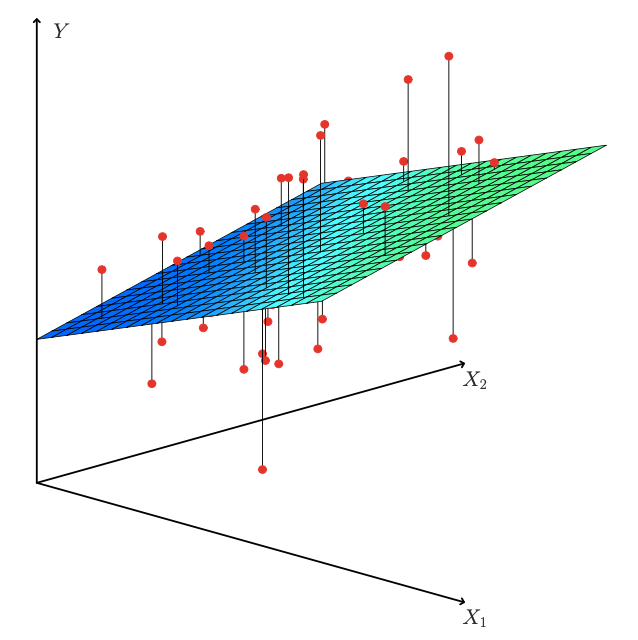
\includegraphics[width=2.59375in,height=\textheight]{images/regression_plane.png}
\end{column}
\end{columns}
\end{frame}

\begin{frame}{Important Questions}
\protect\hypertarget{important-questions}{}
When working with multiple linear regression, we are often interested in
several important questions.

\begin{itemize}
\item
  Is there a relationship between the response and the predictors?
\item
  How well does the model fit the data?
\item
  Given a set of predictor values, what is the predicted response, and
  how accurate is our prediction? We will go over the methods for
  answering each of these questions.
\end{itemize}
\end{frame}

\begin{frame}{Hypothesis Test for Parameters}
\protect\hypertarget{hypothesis-test-for-parameters}{}
One: \emph{Is there a relationship between the response and the
predictors?}

We can address this question by testing whether the regression
coefficients are far enough from zero.

Our null hypothesis and alternative hypothesis are the following: \[
H_{0}: \beta_{1}=\beta_{2}=\cdots=\beta_{p}=0
\hspace{1cm}
H_{a}: \beta_{j} \neq 0 \text{ for some } j
\] The hypothesis can be tested with the
\(\mathbf{F}\)\textbf{-statistic}, which is defined by \[
F=\frac{(\mathrm{TSS}-\mathrm{RSS}) / p}{\mathrm{RSS} /(n-p-1)}.
\] If the \(F\)-statistic is much larger than 1 we reject the null
hypothesis and conclude there is a relationship between at least on the
the predictors and the response. If the \(F\)-statistic is close to 1,
the \(p\)-value can be computed to determine the outcome.
\end{frame}

\begin{frame}{\(RSE\) and \(R^2\)}
\protect\hypertarget{rse-and-r2}{}
Two: \emph{How well does the model fit the data?}

The \(\operatorname{RSE}\) and \(R^2\) are measures of the model fit. In
the multiple linear regression context, \(R^2\) is the square of the
correlation between the response and the fitted linear model. That is,
\(R^2 = \operatorname{Cor}(Y, \hat Y)^2\).

The \(\operatorname{RSE}\) is defined by \[
\mathrm{RSE}=\sqrt{\frac{\mathrm{RSS}}{n-p-1} } \hspace{1cm} \text{where } n = \text{\# observations},\ p = \text{\# predictors}
\]

Important considerations as the number of variables in the model
increases:

\begin{itemize}
\item
  \(R^2\) will increase even if the new variables have a weak
  association with the response.
\item
  \(RSS\) of the training data will decrease, but not necessarily that
  of the testing data.
\item
  \(RSE\) will increase if the decrease in \(RSS\) is small relative to
  the increase in \(p\).
\end{itemize}
\end{frame}

\begin{frame}{Prediction Accuracy}
\protect\hypertarget{prediction-accuracy}{}
Three: \emph{Given a set of predictor values, what is the predicted
response, and how accurate is our prediction?} Once we have fit the
multiple regression model, the response \(Y\) is predicted by \[
        \hat Y = \hat{\beta}_{0}+\hat{\beta}_{1} X_{1}+\cdots+\hat{\beta}_{p} X_{p}.
        \] There are three types of uncertainty associated with the
prediction \(\hat Y\)

\begin{enumerate}
\item
  The \textbf{reducible error} arising from the inaccuracy of the
  coefficient estimates.
\item
  The reducible error stemming from the assumption that the relationship
  between \(Y\) and \(X\) is linear; \textbf{model bias}.
\item
  The \textbf{irreducible error} from the random error associated with
  the true response \(Y = f(x) + \epsilon\).
\end{enumerate}

We can address how much \(Y\) will vary from \(\hat Y\) using prediction
intervals.
\end{frame}

\begin{frame}{Exercises: Multiple Linear Regression}
\protect\hypertarget{exercises-multiple-linear-regression}{}
Open the Linear Regression Exercises R Markdown file.

\begin{itemize}
\tightlist
\item
  Go over the ``Multiple Linear Regression'' section together as a
  class.
\end{itemize}
\end{frame}

\begin{frame}{Qualitative Predictors}
\protect\hypertarget{qualitative-predictors}{}
So far we have only looked at using quantitative predictor variables for
linear regression. However, sometimes the inclusion of qualitative
variables is desirable.

Suppose we have the following information about a set of people:

\begin{itemize}
\item
  \(Y\): income (quantitative: \$ amount)
\item
  \(X_1\): student status (qualitative: is a student or is not)
\item
  \(X_2\): location of residence (qualitative: Toronto, Vancouver,
  Montreal)
\end{itemize}

We want to determine whether there is a relationship between income and
the other two qualitative variables.
\end{frame}

\begin{frame}{Qualitative Predictors: Two Levels}
\protect\hypertarget{qualitative-predictors-two-levels}{}
Let's start by looking at the differences in income between students and
non-students. Our qualitative predictor, or \emph{factor}, has two
levels so we can incorporate into a regression model using a
\textbf{dummy variable} that takes on two possible numerical values.

\[
x_{i}=\left\{\begin{array}{ll}
1 & \text { if } i \text{th person is a student } \\
0 & \text { if } i \text{th person is not a student }
\end{array}\right. 
\]

So we have the following model

\[
y_{i}=\beta_{0}+\beta_{1} x_{i}+\epsilon_{i}=\left\{\begin{array}{ll}
\beta_{0}+\beta_{1}+\epsilon_{i} & \text { if } i \text{th person is a student } \\
\beta_{0}+\epsilon_{i} & \text { if } i \text{th person is not a student }
\end{array}\right.
\]

\begin{itemize}
\item
  \(\beta_0\) is the average income for non-students.
\item
  \(\beta_0 + \beta_1\) is the average income for students.
\end{itemize}

The method for fitting linear models with qualitative predictors using
dummy variables remains the same.
\end{frame}

\begin{frame}{Qualitative Predictors: Multiple Level}
\protect\hypertarget{qualitative-predictors-multiple-level}{}
Now let's look at the difference in income between the residents of
Toronto, Vancouver, and Montreal. We can do this using two dummy
variables.

\[
\begin{aligned}
x_{i 1}&=\left\{\begin{array}{ll}
1 & \text { if } i \text {th person is from Vancouver } \\
0 & \text { if } i \text {th person is not from Vancouver }
\end{array}\right.
\\
x_{i 2}&=\left\{\begin{array}{ll}
1 & \text { if } i \text {th person is from Montreal } \\
0 & \text { if } i \text {th person is not Montreal }
\end{array}\right.
\end{aligned}
\]

The level with no dummy variable is known as the \textbf{baseline}
(Toronto in this example). Our model is now \[
y_{i}=\beta_{0}+\beta_{1} x_{i 1}+\beta_{2} x_{i 2}+\epsilon_{i}=\left\{\begin{array}{ll}
\beta_{0}+\beta_{1}+\epsilon_{i} & \text { if } i \text{th person is from Vancouver } \\
\beta_{0}+\beta_{2}+\epsilon_{i} & \text { if } i \text{th person is from Montreal } \\
\beta_{0}+\epsilon_{i} & \text { if } i \text{th person is from Toronto. }
\end{array}\right.
\]
\end{frame}

\begin{frame}{Qualitative Predictors: Multiple Levels}
\protect\hypertarget{qualitative-predictors-multiple-levels}{}
\[
y_{i}=\beta_{0}+\beta_{1} x_{i 1}+\beta_{2} x_{i 2}+\epsilon_{i}=\left\{\begin{array}{ll}
\beta_{0}+\beta_{1}+\epsilon_{i} & \text { if } i \text{th person is from Vancouver } \\
\beta_{0}+\beta_{2}+\epsilon_{i} & \text { if } i \text{th person is from Montreal } \\
\beta_{0}+\epsilon_{i} & \text { if } i \text{th person is from Toronto. }
\end{array}\right.
\]

The coefficients can be interpreted as

\begin{itemize}
\item
  \(\beta_0\) the average income for people from Toronto
\item
  \(\beta_1\) the difference in the average income between people from
  Vancouver versus Toronto
\item
  \(\beta_2\) the difference in the average income between people from
  Montreal versus Toronto.
\end{itemize}

\begin{enumerate}
\tightlist
\item
  The choice of 0 and 1 as values for the dummy variable or the choice
  of the baseline category are arbitrary and will not change the results
  of the regression
\item
  These choices will impact the interpretation of the coefficients and
  their \(p\)-values.
\item
  Use an F-test to test \(H_0\) : \(\beta_1 = \beta_2 = 0\).
\end{enumerate}
\end{frame}

\begin{frame}{Exercises: Qualitative Predictors}
\protect\hypertarget{exercises-qualitative-predictors}{}
Open the Linear Regression Exercises R Markdown file.

\begin{itemize}
\tightlist
\item
  Go over the ``Qualitative Predictors'' section together as a class.
\end{itemize}
\end{frame}

\begin{frame}{Extensions of the Linear Model}
\protect\hypertarget{extensions-of-the-linear-model}{}
Two of the most important and restrictive assumptions for linear
regression models are

\begin{itemize}
\tightlist
\item
  The relationship between the predictors and the response is
  \alert{additive}.

  \begin{itemize}
  \tightlist
  \item
    \(\Rightarrow\) \emph{The association between a predictor and the
    response does not depend on any of the other predictors.}
  \end{itemize}
\item
  The relationship between the predictors and the response is
  \alert{linear}.

  \begin{itemize}
  \tightlist
  \item
    \(\Rightarrow\) \emph{A one-unit change in a predictor induces a
    constant change in the response regardless of the value of the
    predictor.}
  \end{itemize}
\end{itemize}

We will examine the relaxation of the additive assumption but
modifications to the linear assumption will be left until section 6.6.
\end{frame}

\begin{frame}{Removing the Additive Assumption}
\protect\hypertarget{removing-the-additive-assumption}{}
Consider the following linear regression model with two predictors \[
Y=\beta_{0}+\beta_{1} X_{1}+\beta_{2} X_{2}+\epsilon
\] We can include the product of \(X_1\) and \(X_2\) as a third
predictor called the \textbf{interaction term}.
\[Y=\beta_{0}+\beta_{1} X_{1}+\beta_{2} X_{2}+\alert{\beta_{3} X_{1} X_{2}}+\epsilon\]
This means that a change in the value of \(X_2\) will change the
association between \(X_1\) and \(Y\).

We can look at the \(p\)-value for \(H_0: \beta_3 = 0\) to determine
whether the interaction term is justified.

The \textbf{hierarchical principal}: when including an interaction in a
model, the main effects should also be included even if the \(p\)-values
for these coefficients are not significant.
\end{frame}

\begin{frame}{Exercises: Interaction Term}
\protect\hypertarget{exercises-interaction-term}{}
Open the Linear Regression Exercises R Markdown file.

\begin{itemize}
\tightlist
\item
  Go over the ``Interaction Term'' section together as a class.
\end{itemize}
\end{frame}

\begin{frame}{Potential Problems}
\protect\hypertarget{potential-problems}{}
There are quite a few problems that can arise when fitting a linear
regression model to a data set.

\begin{itemize}
\item
  Non-linear response-predictor relationship
\item
  Correlation of error terms
\item
  Non-constant variance of error terms
\item
  Outliers
\item
  High-leverage points
\end{itemize}

We will briefly explain how to identify these problems but we will wait
to provide solutions until later sections within this module.
\end{frame}

\begin{frame}{Non-Linearity}
\protect\hypertarget{non-linearity}{}
Linear regression assumes a linear relationship between the predictors
and the response. If this assumption is invalid then conclusions derived
from the model are flawed.

Identification:

\begin{itemize}
\item
  Plot the residuals \(e_i = y_i - \hat y_i\) versus the predictor
  \(x_i\) (or versus \(y_i\) in the case of multiple regression)
\item
  There should be no discernible pattern in the residuals, otherwise
  this may indicate non-linearity.
\end{itemize}
\end{frame}

\begin{frame}{Non-Linearity}
\protect\hypertarget{non-linearity-1}{}
Plot of the residuals versus the predicted values for a linear
regression fit to a dataset.

\begin{figure}

{\centering 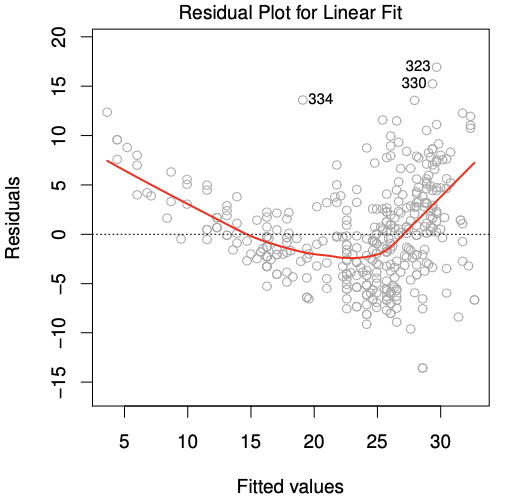
\includegraphics[width=2.22917in,height=\textheight]{images/residuals-01.png}

}

\end{figure}

There is a clear trend in the residuals illustrated by the red curve
which could indicate patterns in the data that are not captured by the
linear model.
\end{frame}

\begin{frame}{Correlation of Errors}
\protect\hypertarget{correlation-of-errors}{}
Linear regression assumes that the error terms
\(\epsilon_{1}, \epsilon_{2}, \ldots, \epsilon_{n}\) are uncorrelated
(i.e.~the value of \(\epsilon_{i}\) is unrelated to the value for
\(\epsilon_{i+1}\)). If this is violated, the estimated standard errors
are much smaller than the truth, leading to unwarranted confidence in
the model.

Examples

\begin{itemize}
\item
  correlation between consecutive observations in time series data.
\item
  observations are related in some other way (ex: individuals are
  members of the same family or have been exposed to the same
  environmental factors).
\end{itemize}

Identification for time series:

\begin{itemize}
\item
  Plot residuals versus time.
\item
  Look for temporal patterns that could indicated correlation of error
  terms.
\end{itemize}
\end{frame}

\begin{frame}{Correlation of Errors}
\protect\hypertarget{correlation-of-errors-1}{}
Both plots show the residuals from a linear regression fit to time
series data versus time. The top plot shows no correlation between the
residuals whereas the bottom plot clearly has a time dependent
structure.

\begin{figure}

{\centering 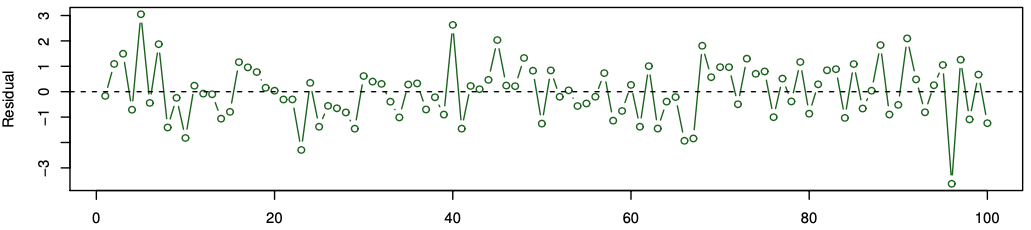
\includegraphics[width=4.66667in,height=\textheight]{images/uncorrelated_error.png}

}

\end{figure}

\begin{figure}

{\centering 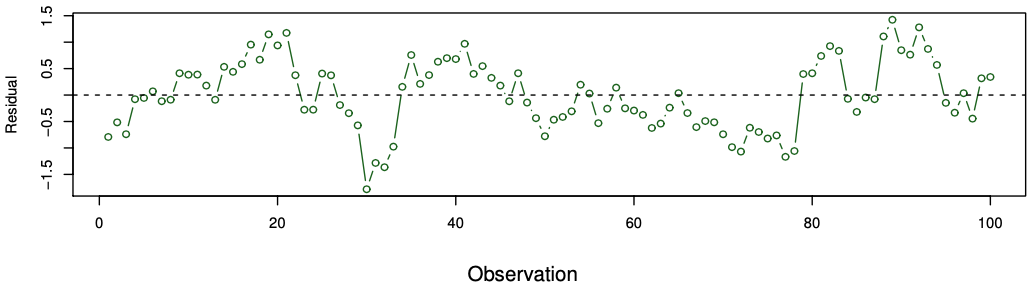
\includegraphics[width=4.66667in,height=\textheight]{images/correlated_error.png}

}

\end{figure}
\end{frame}

\begin{frame}{Non-Constant Variance of Errors}
\protect\hypertarget{non-constant-variance-of-errors}{}
Linear regression also assumes constant variance of the error terms,
\(\operatorname{Var}(\epsilon_i) = \sigma^2\). If this assumption is
invalid, the standard errors, confidence intervals, and hypothesis tests
for the linear model are undermined.

Identification:

\begin{enumerate}
\item
  Plot the residuals versus the response.
\item
  Look for a funnel shape in the plot (this indicates an increase or
  decrease in the variance of the errors as a function of the response)
\end{enumerate}
\end{frame}

\begin{frame}{Non-Constant Variance of Errors}
\protect\hypertarget{non-constant-variance-of-errors-1}{}
Plot for the residuals versus the fitted values of a linear regression
model.

\begin{figure}

{\centering 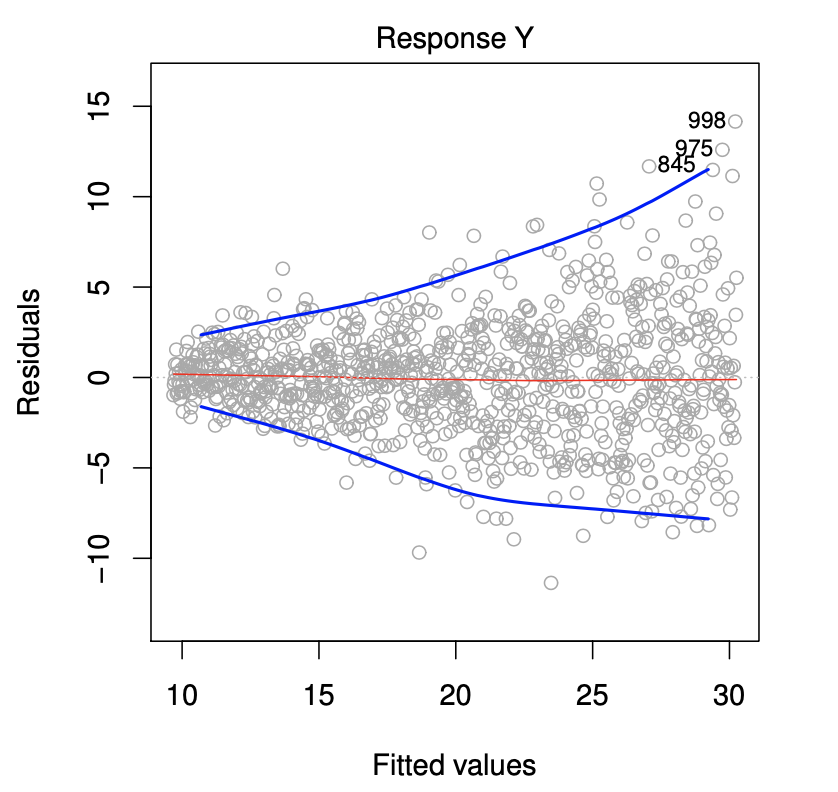
\includegraphics[width=2.20833in,height=\textheight]{images/variance_errors.png}

}

\end{figure}

The residuals show a clear funnel shape with increasing response values
resulting in increasing variance of the error terms.
\end{frame}

\begin{frame}{Outliers}
\protect\hypertarget{outliers}{}
\textbf{Outliers} are data points that have unusual values for \(y_i\)
given an unremarkable \(x_i\). That is, \(y_i\) is far from the value
predicted by the model for \(x_i\). Outliers can occur as a result of an
error in data collection or a variety of other reasons.

Outliers often have little effect on the parameter fitting, but they can
alter the \(RSE\) and \(R^2\) which can impact the interpretation of the
fit.

Identification:

\begin{enumerate}
\item
  Plot the \textbf{studentized residuals} which are computed by dividing
  the residuals \(e_i\) by the estimated standard error.
\item
  Observations with studentized residuals greater than 3 or less than -3
  are probably outliers.
\end{enumerate}
\end{frame}

\begin{frame}{Outliers}
\protect\hypertarget{outliers-1}{}
Plot of the studentized residuals versus the response values.

\begin{figure}

{\centering 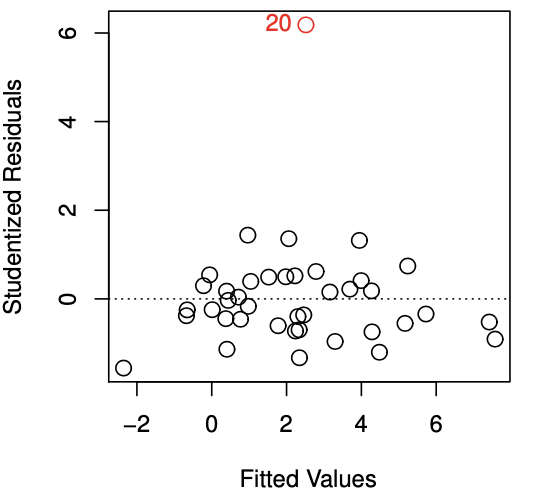
\includegraphics[width=2.34375in,height=\textheight]{images/studentized_re.png}

}

\end{figure}

The red point at the top of the plot is above 3 which indicates it is an
outlier.
\end{frame}

\begin{frame}{High Leverage Points}
\protect\hypertarget{high-leverage-points}{}
\textbf{High leverage points} are observations that have an unusual
predictor value. These points tend to impact the fitted regression quite
a bit and are therefore very important to identify.

Identification:

\begin{itemize}
\item
  In simple linear regression, look for observations with a predictor
  value that is far outside the range of the rest.
\item
  In multiple regression, we are looking for an unusual combination of
  predictors which can be harder to identify

  \begin{itemize}
  \item
    Compute the leverage statistic for each observation.
  \item
    If the leverage statistic is much greater than \((p+1)n\), the
    observation may have high leverage.
  \end{itemize}
\end{itemize}
\end{frame}

\begin{frame}{High Leverage Points}
\protect\hypertarget{high-leverage-points-1}{}
The left plot shows the response versus the predictors for a simple
linear regression. The right plot show the studentized residuals versus
the leverage.

\begin{columns}[T]
\begin{column}{0.5\textwidth}
\begin{figure}

{\centering 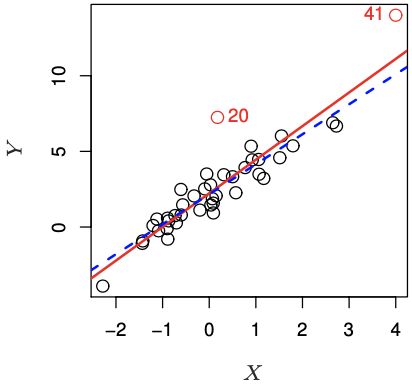
\includegraphics[width=1.32292in,height=\textheight]{images/simple_leverage.png}

}

\end{figure}
\end{column}

\begin{column}{0.5\textwidth}
\begin{figure}

{\centering 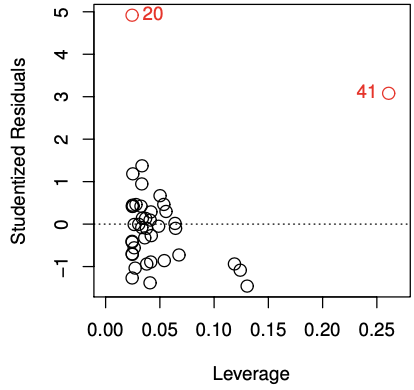
\includegraphics[width=1.32292in,height=\textheight]{images/multiple_leverage.png}

}

\end{figure}
\end{column}
\end{columns}

Observation 41 in the left plot has a very large predictor value which
indicates it is a high leverage point. This is confirmed in the right
plot by the leverage index. The right plot also indicates 41 has a
larger studentized residual (as does observation 20) so 41 is an outlier
and a high leverage point.
\end{frame}

\begin{frame}{Exercises}
\protect\hypertarget{exercises}{}
Open the Linear Regression Exercises R Markdown file.

\begin{itemize}
\item
  Go over the ``Helpful Plots'' section together as a class.
\item
  Complete the exercises at the end of the file.
\end{itemize}
\end{frame}

\begin{frame}{References}
\protect\hypertarget{references}{}
Chapter 3 of the ISLR2 book:

James, Gareth, et al.~``Linear Regression.'' An Introduction to
Statistical Learning: with Applications in R, 2nd ed., Springer, 2021.
\end{frame}



\end{document}
